

Finda a construção dos indicadores apresentados no Capítulo \ref{ch:cap5}, tinha-se como o objetivo a automatização do processo de aplicação destes indicadores a todos os novos contratos adicionados diariamente à base de dados. Este processo foi aplicado aos concursos públicos e foram utilizadas todas as flags, exceto a R031 e R051. Primeiramente, construiu-se uma nova tabela, chamada \textit{daily\_flags}, com a configuração da Tabela \ref{tab:dailyexample}. 


\begin{table}[H]
	\centering
	\renewcommand{\arraystretch}{1.15}
	\setlength{\tabcolsep}{15pt}
	\resizebox{\textwidth}{!}{%
		\begin{tabular}{lllllllll}
			\toprule
			\textbf{ID}                  & \textbf{Data Publicação}       & \textbf{Verificação}     & \textbf{RF2}              & \textbf{RF3}              & \textbf{R003}             & \textbf{R017}            & \textbf{R018}             & \textbf{R019}            \\ \midrule
			\multicolumn{1}{c}{12345678} & \multicolumn{1}{c}{01/01/2024} & \multicolumn{1}{c}{true} & \multicolumn{1}{c}{false} & \multicolumn{1}{c}{false} & \multicolumn{1}{c}{false} & \multicolumn{1}{c}{true} & \multicolumn{1}{c}{false} & \multicolumn{1}{c}{true} \\ \bottomrule
		\end{tabular}%
	}
	\caption{Exemplo de aplicação de todos os indicadores binários a um concurso público.}
	\label{tab:dailyexample}
\end{table}

Esta tabela é constituída pelo identificador do contrato, a data de publicação, uma coluna de verificação cujo propósito irá ser clarificado nos próximos parágrafos e as colunas referentes a cada uma das flags. Este processo consistiu em selecionar, diariamente, os novos concursos públicos adicionados à tabela principal \textit{contratos\_basegov}, copiar as colunas que contém o identificador e a data de publicação dos mesmos, aplicar as flags e inserir o output, de cada flag para cada contrato, nesta nova tabela. Para tal, foi necessário dividir este processo em várias etapas distintas. Na Figura \ref{fig:esquema} é possível observar um esquema que retrata de uma forma macroscópica este processo.  


\begin{figure}[H]
	\centering
	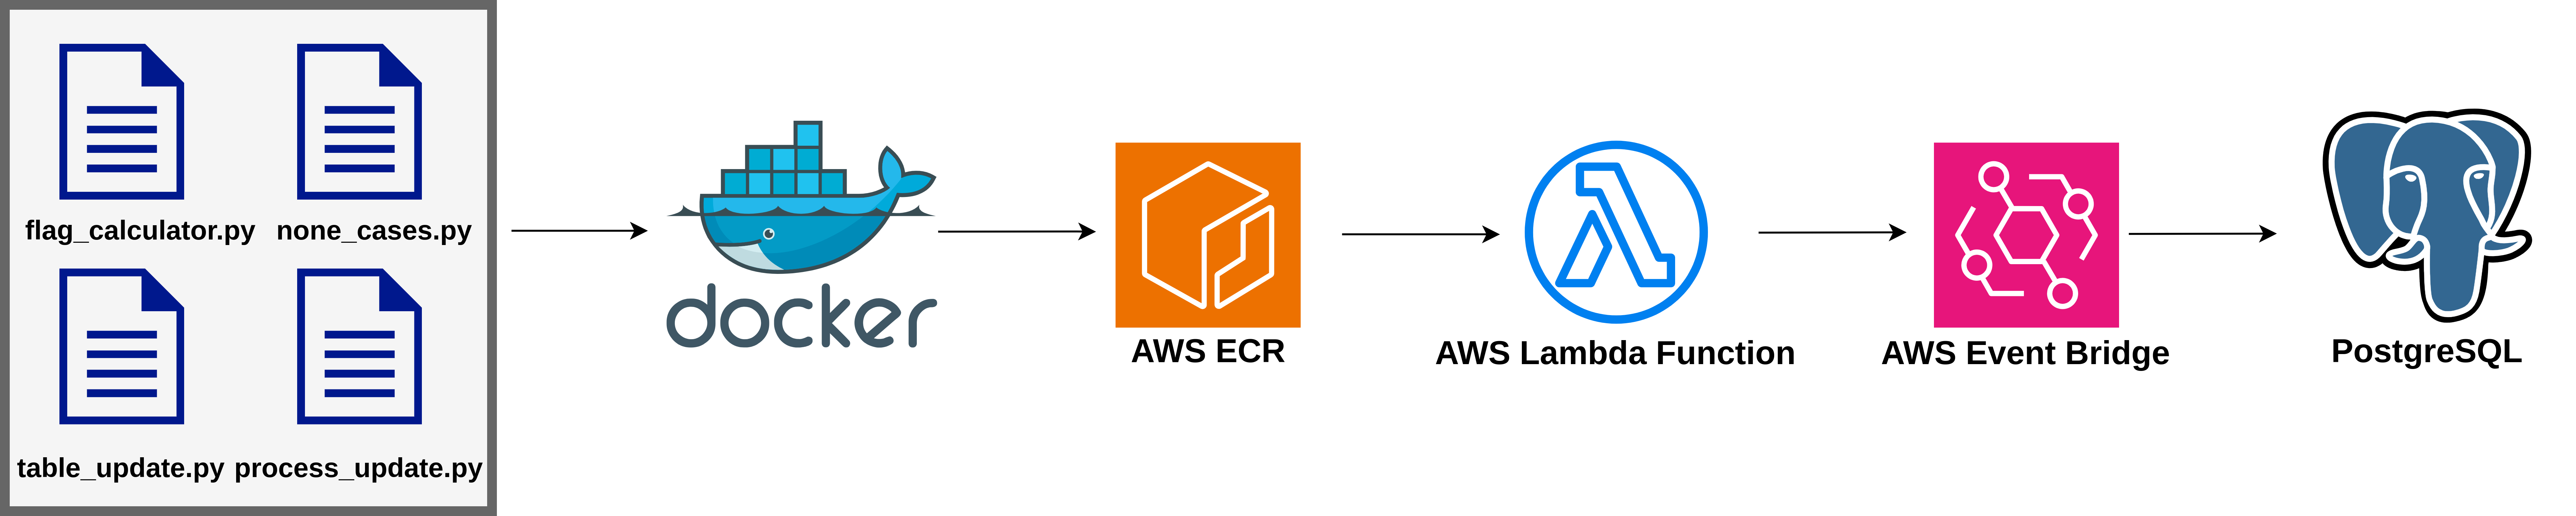
\includegraphics[width=\textwidth]{imagens/daily_flags_v2.png}
	\caption{Esquema do processo de automatização.}
	\label{fig:esquema}
\end{figure}


Na base deste procedimento estão quatro ficheiros \textit{python} desenvolvidos, cada um deles com um objetivo específico. No ficheiro table\_update.py são definidas as funções responsáveis por atualizar e realizar as operações necessárias na tabela auxiliar \textit{concursos\_publicos}. Começa-se por verificar qual é o id do último contrato desta tabela, a fim de não copiar contratos já existentes. De seguida, são copiadas as colunas \textit{id}, \textit{data\_publicacao}, 	\textit{contractTypes}, \textit{fundamentacao}, \textit{entidade\_adjudicante}, \textit{entidades\_contratadas}, \textit{entidades\_concorrentes}, \textit{executionPlace}, \textit{cpv} e \textit{preco\_contratual} dos novos contratos da tabela original. Após copiar os novos contratos, são efetuadas todas as operações auxiliares necessárias:

\begin{my_enumerate}
	
	\item Fazer a separação das colunas \textit{entidade\_adjudicante} e \textit{entidades\_contratadas} tal como foi demonstrado na secção \ref{ch:entis}.
	
	\item Fazer o cálculo do número de entidades concorrentes tal como foi demonstrado na secção \ref{ch:entis}.
	
	\item Fazer a classificação dos contratos de acordo com a tipologia: Bens e Serviços / Empreitadas.
			
\end{my_enumerate}



No \textit{script} flag\_calculator.py são definidas todas as funções, usando a biblioteca psycopg2 que permite fazer a conexão entre o python e o postgreSQL, responsáveis por calcular as flags presentes na Tabela \ref{tab:dailyexample}. De seguida, foi criada uma função global que incorpora todas as funções de cálculo das flags e que atribui, para cada coluna das flags, a string \textit{true} para contratos inconformes. Caso contrário, é atribuída a string \textit{false}. No ficheiro process\_update.py são invocadas todas as funções desenvolvidas nos ficheiros flag\_calculator.py e table\_update.py. Aqui, começa-se por aplicar as funções desenvolvidas no primeiro ficheiro e, só de seguida, as do último. No fim do processo de cálculo das flags é atribuído um valor \textit{true} na coluna de verificação. Esta coluna serve como um mecanismo de prevenção para a eventualidade de o processo não decorrer como suposto. Quando ocorre alguma anomalia e este processo não decorre como planeado, a coluna da verificação contém o valor \textit{false}. Nessas situações são invocadas as funções do script \textit{none\_cases.py}. Primeiramente, são identificadas todas as entradas que contenham o valor \textit{false} nesta coluna. De seguida, procede-se à remoção das mesmas e, por fim, repete-se o processo descrito no parágrafo anterior.

Após a construção destes ficheiros, foi criada uma imagem em Docker com os mesmos. De seguida, no serviço de cloud AWS, foi criado um repositório, num Elastic Container Register (ECR), onde se armazenou a imagem Docker. Para executar os ficheiros presentes nesta imagem, foi criada uma função Lambda que guarda o output na tabela \textit{daily\_flags} da base de dados. Por fim, de forma a executar este processo de forma diária, foi programada uma calendarização do mesmo através do AWS Event Bridge. 

























